\documentclass[10pt]{beamer}

\usetheme{metropolis}
\usepackage{appendixnumberbeamer}

\usepackage{booktabs}
\usepackage[scale=2]{ccicons}

\usepackage{pgfplots}
\usepgfplotslibrary{dateplot}

\usepackage{xspace}
\newcommand{\themename}{\textbf{\textsc{metropolis}}\xspace}

\usepackage{ctex,listings}
\title{Project4: File Systems}
\subtitle{PintOS}
\date{\today}
\author{陈震雄}
\institute{武汉大学}
% defs
\def\cmd#1{\texttt{\color{red}\footnotesize $\backslash$#1}}
\def\env#1{\texttt{\color{blue}\footnotesize #1}}

\definecolor{deepblue}{rgb}{0,0,0.5}
\definecolor{deepred}{rgb}{0.6,0,0}
\definecolor{deepgreen}{rgb}{0,0.5,0}
\definecolor{halfgray}{gray}{0.55}

\lstset{
    basicstyle=\ttfamily\tiny,
    keywordstyle=\bfseries\color{deepblue},
    emphstyle=\ttfamily\color{deepred},
    stringstyle=\color{deepgreen},
    numbers=left,
    numberstyle=\tiny\color{halfgray},
    showspaces=false,
    commentstyle=\color{halfgray}
}

\titlegraphic{\hfill
\includegraphics[height=2cm]{figures/whulogo.pdf}}

\logo{
\includegraphics[height=1cm]{figures/whulogo.pdf}}
\begin{document}

\maketitle

\begin{frame}{Table of contents}
  \setbeamertemplate{section in toc}[sections numbered]
  \tableofcontents[hideallsubsections]
\end{frame}
%----------------
\section{Introduction}
\begin{frame}[fragile]{Introduction}
    In the previous two assignments, you made extensive use of a file system without actually worrying about how it was implemented underneath. For this last assignment, you will \textbf{improve the implementation of the file system.}
\end{frame}
%---------Task3---------------
\section{Task 3: Buffer Cache}
\begin{frame}[fragile]{Exercise 3.1}
    \textbf{Modify the file system to keep a cache of file blocks.}

When a request is made to read or write a block, \textbf{check to see if it is in the cache}, and if so, use the cached data without going to disk.

Otherwise, \textbf{fetch the block from disk into the cache}, evicting an older entry if necessary.

\textbf{You are limited to a cache no greater than 64 sectors in size}.

\textbf{Implement buffer cache and cache replacement algorithm.}

\textbf{You must implement a cache replacement algorithm that is at least as good as the "clock" algorithm.}

\textbf{write-behind,read-ahead}
\end{frame}
%-----------------------------
\begin{frame}[fragile]{Data structure}
\begin{lstlisting}[language=C]
struct disk_cache 
{    
    uint8_t block[BLOCK_SECTOR_SIZE];   /**< 512 Bytes */
    block_sector_t disk_sector;         /**< disk sector */

    bool is_free;                       /**< is free */
    int open_cnt;                       /**< open count */
    bool accessed;                      /**< accessed */
    bool dirty;                         /**< dirty */  
};

struct lock cache_lock;                 /**< cache lock */
struct disk_cache cache_array[64];      /**< cache array */
\end{lstlisting}
\end{frame}
%-----------------------------
\begin{frame}[fragile]{Read}
\begin{columns}
\begin{column}{0.5\textwidth}
\begin{lstlisting}[language=C]
int access_cache_entry(block_sector_t 
disk_sector, bool dirty) {
  lock_acquire(&cache_lock);
  int idx = get_cache_entry(disk_sector);
  if(idx == -1)
    idx = replace_cache_entry(disk_sector, dirty);
  else {
    cache_array[idx].open_cnt++;
    cache_array[idx].accessed = true;
    cache_array[idx].dirty |= dirty;
  }
  lock_release(&cache_lock);
  return idx;
}

int replace_cache_entry(block_sector_t
disk_sector, bool dirty)
{
  int idx = get_free_entry();
  int i = 0;
  if(idx == -1) /**< cache is full. */
  {
    for(i = 0; ; i = (i + 1) % CACHE_MAX_SIZE)
    {
      if(cache_array[i].open_cnt > 0)
        continue;
      if(cache_array[i].accessed == true)
        cache_array[i].accessed = false;
\end{lstlisting}
\end{column}
\begin{column}{0.5\textwidth}
\begin{lstlisting}[language=C]
  /* evict it */
      else
      {
        /* write back */
        if(cache_array[i].dirty == true)
        {
          block_write(fs_device, 
          cache_array[i].disk_sector,
            &cache_array[i].block);
        }

        init_entry(i);
        idx = i;
        break;
      }
    }
  }
  cache_array[idx].disk_sector = disk_sector;
  cache_array[idx].is_free = false;
  cache_array[idx].open_cnt++;
  cache_array[idx].accessed = true;
  cache_array[idx].dirty = dirty;
  block_read(fs_device,
  cache_array[idx].disk_sector, 
  &cache_array[idx].block);
  return idx;
}
\end{lstlisting}
\end{column}
\end{columns}
\end{frame}
%-----------------------------
\begin{frame}[fragile]{Write}
\begin{lstlisting}[language=C]
void 
write_back(bool clear)
{
    int i;
    lock_acquire(&cache_lock);

    for(i = 0; i < CACHE_MAX_SIZE; i++)
    {
        if(cache_array[i].dirty == true)
        {
            block_write(fs_device, cache_array[i].disk_sector, &cache_array[i].block);
            cache_array[i].dirty = false;
        }

        /* clear cache line (filesys done) */
        if(clear) 
          init_entry(i);
    }

    lock_release(&cache_lock);
}
\end{lstlisting}
\end{frame}
%----------------------
\begin{frame}[fragile]{Read-ahead and Write -behind}
\begin{lstlisting}[language=C]
// Write-behind
void init_cache(void) {
  int i;
  lock_init(&cache_lock);
  for(i = 0; i < CACHE_MAX_SIZE; i++)
    init_entry(i);
  thread_create("cache_writeback", PRI_MIN, func_periodic_writer, NULL);
}
// Read-ahead
void func_read_ahead(void *aux) {
    block_sector_t disk_sector = *(block_sector_t *)aux;
    lock_acquire(&cache_lock);

    int idx = get_cache_entry(disk_sector);

    /* need eviction */
    if (idx == -1)
        replace_cache_entry(disk_sector, false);
    
    lock_release(&cache_lock);
    free(aux);
}

void ahead_reader(block_sector_t disk_sector) {
    block_sector_t *arg = malloc(sizeof(block_sector_t));
    *arg = disk_sector + 1;  /**< next block */
    thread_create("cache_read_ahead", PRI_MIN, func_read_ahead, arg);
}

\end{lstlisting}
\end{frame}
%---------Task1----------------
\section{Task 1: Indexed and Extensible Files}
%----------------------
\begin{frame}[fragile]{Exercise 1.1}
    \textbf{The basic file system allocates files as a single extent}, making it vulnerable to \textbf{external fragmentation}, that is, it is possible that an n-block file cannot be allocated even though n blocks are free.

\textbf{Eliminate this problem by modifying the on-disk inode structure.} In practice, this probably means \textbf{using an index structure with direct, indirect, and doubly indirect blocks.}

\textbf{Modify inode structure to accommodate external fragmentation.}
\end{frame}
%-----------------------
\begin{frame}[fragile]{Data Structure}
\begin{lstlisting}[language=C]
struct inode_disk
  {
    off_t length;                       /**< File size in bytes. */
    unsigned magic;                     /**< Magic number. */
    uint32_t unused[107];               /**< Not used. */

    uint32_t direct_index;              /**< Number of direct blocks. */
    uint32_t indirect_index;            /**< Number of indirect blocks. */
    uint32_t double_indirect_index;     /** Number of double indirect blocks. */
    block_sector_t blocks[14];          /**< Block pointers. */
    bool is_dir;                        /** True if directory. */
    block_sector_t parent;              /** Parent block sector. */
  };
struct inode 
  {
    struct list_elem elem;              /**< Element in inode list. */
    block_sector_t sector;              /**< Sector number of disk location. */
    int open_cnt;                       /**< Number of openers. */
    bool removed;                       /**< True if deleted, false otherwise. */
    int deny_write_cnt;                 /**< 0: writes ok, >0: deny writes. */

    off_t length;                       /**< File size in bytes. */
    off_t read_length;                  /** File size in bytes. */
    uint32_t direct_index;              /**< Number of direct blocks. */
    uint32_t indirect_index;            /**< Number of indirect blocks. */
    uint32_t double_indirect_index;     /** Number of double indirect blocks. */
    block_sector_t blocks[14];          /** Block pointers. */
    bool is_dir;                        /** True if directory. */
    block_sector_t parent;              /** Parent block sector. */
    struct lock lock;                   /** Lock for inode. */
  };
\end{lstlisting}
\end{frame}
%----------------------
\begin{frame}[fragile]{Inode create}
\begin{columns}
\begin{column}{0.5\textwidth}
\begin{lstlisting}[language=C]
bool
inode_create (block_sector_t sector, off_t length, bool is_dir)
{
  struct inode_disk *disk_inode = NULL;
  bool success = false;

  ASSERT (length >= 0);

  /* If this assertion fails, 
  the inode structure is not exactly
  one sector in size, and you should fix that. */
  ASSERT (sizeof *disk_inode == BLOCK_SECTOR_SIZE);

  disk_inode = calloc (1, sizeof *disk_inode);
  if (disk_inode != NULL)
    {
      /* ADDED */
      disk_inode->length = length;
      disk_inode->magic = INODE_MAGIC;
      disk_inode->is_dir = is_dir;
      disk_inode->parent = ROOT_DIR_SECTOR;
      if (inode_alloc(disk_inode)) 
        {
          block_write (fs_device, sector, disk_inode);
          success = true; 
        } 
      free (disk_inode);
    }
  return success;
}
\end{lstlisting}
\end{column}
\begin{column}{0.5\textwidth}
\begin{lstlisting}[language=C]
bool
inode_alloc (struct inode_disk *inode_disk)
{
  struct inode inode;
  inode.length = 0;
  inode.direct_index = 0;
  inode.indirect_index = 0;
  inode.double_indirect_index = 0;

  inode_grow(&inode, inode_disk->length);
  inode_disk->direct_index = inode.direct_index;
  inode_disk->indirect_index = inode.indirect_index;
  inode_disk->double_indirect_index = 
  inode.double_indirect_index;
  memcpy(&inode_disk->blocks, &inode.blocks,
  INODE_PTRS * sizeof(block_sector_t));
  return true;
}
\end{lstlisting}
\end{column}
\end{columns}
\end{frame}
%-----------------------
\begin{frame}[fragile]{Inode grow}
\begin{columns}
\begin{column}{0.5\textwidth}
\begin{lstlisting}[language=C]
off_t
inode_grow (struct inode *inode, off_t length)
{
  static char zeros[BLOCK_SECTOR_SIZE];
  size_t grow_sectors = bytes_to_sectors(length) - 
  bytes_to_sectors(inode->length);
  if (grow_sectors == 0)
    return length;

  /* direct blocks (index < 4) */
  while (inode->direct_index < DIRECT_BLOCKS
  && grow_sectors != 0)
  {
    if (!free_map_allocate(1, &inode->
    blocks[inode->direct_index])) {
      return -1; /**< Allocation failed */
    }
    block_write(fs_device, inode->
    blocks[inode->direct_index], zeros);
    inode->direct_index++;
    grow_sectors--;
  }
\end{lstlisting}
\end{column}
\begin{column}{0.5\textwidth}
\begin{lstlisting}[language=C]
/* indirect blocks (index < 13) */
  while (inode->direct_index < (int) DIRECT_BLOCKS 
  + INDIRECT_BLOCKS && grow_sectors != 0)
  {
    block_sector_t blocks[128];
    if (inode->indirect_index == 0) {
      if (!free_map_allocate(1, &inode->
      blocks[inode->direct_index])) {
        return -1;
      }
    } else {
      block_read(fs_device, inode->
      blocks[inode->direct_index], &blocks);
    }
    while (inode->indirect_index < 
    INDIRECT_PTRS && grow_sectors != 0)
    {
      if (!free_map_allocate(1, 
      &blocks[inode->indirect_index])) {
        return -1;
      }
      block_write(fs_device, 
      blocks[inode->indirect_index], zeros);
      inode->indirect_index++;
      grow_sectors--;
    }
    block_write(fs_device, inode->
    blocks[inode->direct_index], &blocks);
    if (inode->indirect_index 
    == INDIRECT_PTRS) {
      inode->indirect_index = 0;
      inode->direct_index++;
    }
  }
\end{lstlisting}
\end{column}
\end{columns}
\end{frame}
%--------------------
\begin{frame}[fragile]{Inode grow}
\begin{lstlisting}[language=C]
if (inode->direct_index == INODE_PTRS - 1 && grow_sectors != 0) {
    block_sector_t level_one[128];
    block_sector_t level_two[128];
    if (inode->double_indirect_index == 0 && inode->indirect_index == 0) {
      if (!free_map_allocate(1, &inode->blocks[inode->direct_index]))
        return -1;
    } else 
      block_read(fs_device, inode->blocks[inode->direct_index], &level_one);
    while (inode->indirect_index < INDIRECT_PTRS && grow_sectors != 0) {
      if (inode->double_indirect_index == 0) {
        if (!free_map_allocate(1, &level_one[inode->indirect_index])) {
          return -1;
        }
      } else
        block_read(fs_device, level_one[inode->indirect_index], &level_two);
      while (inode->double_indirect_index < INDIRECT_PTRS && grow_sectors != 0) {
        if (!free_map_allocate(1, &level_two[inode->double_indirect_index])) {
          return -1;
        }
        block_write(fs_device, level_two[inode->double_indirect_index], zeros);
        inode->double_indirect_index++;
        grow_sectors--;
      }
      block_write(fs_device, level_one[inode->indirect_index], &level_two);
      if (inode->double_indirect_index == INDIRECT_PTRS) {
        inode->double_indirect_index = 0;
        inode->indirect_index++;
      }
    }
    block_write(fs_device, inode->blocks[inode->direct_index], &level_one);
  }
  return length;
}
\end{lstlisting}
\end{frame}
%--------------------
\begin{frame}[fragile]{read}
\begin{columns}
\begin{column}{0.5\textwidth}
\begin{lstlisting}[language=C]
off_t
inode_read_at (struct inode *inode, void *buffer_, off_t size, off_t offset) 
{
  uint8_t *buffer = buffer_;
  off_t bytes_read = 0;

  off_t length = inode->read_length;

  if(offset >= length)
    return 0;

  while (size > 0) 
    {
      /* Disk sector to read, 
      starting byte offset within sector. */
      block_sector_t sector_idx = 
      byte_to_sector (inode, length, offset);
      int sector_ofs = offset % BLOCK_SECTOR_SIZE;

      /* Bytes left in inode,
      bytes left in sector, lesser of the two. */
      off_t inode_left = length - offset;
      int sector_left = 
      BLOCK_SECTOR_SIZE - sector_ofs;
      int min_left = inode_left < sector_left ? inode_left : sector_left;
\end{lstlisting}
\end{column}
\begin{column}{0.5\textwidth}
\begin{lstlisting}[language=C]
      /* Number of bytes to actually 
      copy out of this sector. */
      int chunk_size = size < min_left ? size : min_left;
      if (chunk_size <= 0)
        break;

      int cache_idx = 
      access_cache_entry(sector_idx, false);
      memcpy(buffer + bytes_read, 
       cache_array[cache_idx].block + sector_ofs,
       chunk_size);
      cache_array[cache_idx].accessed = true;
      cache_array[cache_idx].open_cnt--;     
      /* Advance. */
      size -= chunk_size;
      offset += chunk_size;
      bytes_read += chunk_size;
    }
  return bytes_read;
}
\end{lstlisting}
\end{column}
\end{columns}
\end{frame}
%--------------------
\begin{frame}[fragile]{Inode write}
\begin{columns}
\begin{column}{0.5\textwidth}
\begin{lstlisting}[language=C]
off_t
inode_write_at (struct inode *inode, const void 
*buffer_, off_t size, off_t offset) 
{
  const uint8_t *buffer = buffer_;
  off_t bytes_written = 0;

  if (inode->deny_write_cnt)
    return 0;

  /* beyond EOF, need extend */
  if(offset + size > inode_length(inode))
  {
    /* no sync required for dirs */
    if(!inode->is_dir)
      lock_acquire(&inode->lock);

    inode->length = inode_grow(inode, offset + size);

    if(!inode->is_dir)
      lock_release(&inode->lock);
  }

  while (size > 0) 
    {
\end{lstlisting}
\end{column}
\begin{column}{0.5\textwidth}
\begin{lstlisting}[language=C]
      block_sector_t sector_idx = byte_to_sector
      (inode, inode_length(inode),
       offset);
      int sector_ofs = offset % BLOCK_SECTOR_SIZE;
      off_t inode_left = inode_length (inode) - 
      offset;
      int sector_left = BLOCK_SECTOR_SIZE - 
      sector_ofs;
      int min_left = inode_left < sector_left ? 
      inode_left : sector_left;

      int chunk_size = size < min_left ? size : 
      min_left;
      if (chunk_size <= 0)
        break;
      int cache_idx = access_cache_entry(sector_idx, 
      true);
      memcpy(cache_array[cache_idx].block + 
      sector_ofs, buffer + bytes_written, chunk_size);
      cache_array[cache_idx].accessed = true;
      cache_array[cache_idx].dirty = true;
      cache_array[cache_idx].open_cnt--;
      /* Advance. */
      size -= chunk_size;
      offset += chunk_size;
      bytes_written += chunk_size;
    }

  inode->read_length = inode_length(inode);
  return bytes_written;
}
\end{lstlisting}
\end{column}
\end{columns}
\end{frame}
%---------------------
\begin{frame}[fragile]{Other funcs}
\begin{lstlisting}[language=C]
struct bitmap;

void inode_init (void);
bool inode_create (block_sector_t, off_t, bool);
struct inode *inode_open (block_sector_t);
struct inode *inode_reopen (struct inode *);
block_sector_t inode_get_inumber (const struct inode *);
void inode_close (struct inode *);
void inode_remove (struct inode *);
off_t inode_read_at (struct inode *, void *, off_t size, off_t offset);
off_t inode_write_at (struct inode *, const void *, off_t size, off_t offset);
void inode_deny_write (struct inode *);
void inode_allow_write (struct inode *);
off_t inode_length (const struct inode *);
bool inode_is_dir (const struct inode *);
block_sector_t inode_get_parent (const struct inode *);

/* ADDED */
bool inode_is_dir (const struct inode *);
int inode_get_open_cnt (const struct inode *);
block_sector_t inode_get_parent (const struct inode *);
bool inode_set_parent (block_sector_t parent, block_sector_t child);
void inode_lock (const struct inode *inode);
void inode_unlock (const struct inode *inode);

/* ADDED */
bool inode_alloc (struct inode_disk *inode_disk);
off_t inode_grow (struct inode* inode, off_t length);
void inode_free (struct inode *inode)
\end{lstlisting}
\end{frame}
%--------------------
\section{Task 2: Subdirectories}
\begin{frame}[fragile]{Exercise 2.1}
\textbf{Implement a hierarchical name space.
}
In the basic file system, all files live in a \textbf{single} directory.

Modify this to allow directory entries to point to files or to other directories.

\textbf{Implement a hierarchical name space.}

In the basic file system, all files live in a single directory.

Modify this to allow directory entries to point to files or to other directories.
\end{frame}
\begin{frame}[fragile]{dir\_add and other funcs}
\begin{lstlisting}[language=C]
bool
dir_add (struct dir *dir, const char *name, block_sector_t inode_sector)
{
    ...
  /* set parent of added file to this dir */
  if (!inode_set_parent(inode_get_inumber(dir_get_inode(dir)), inode_sector))
    goto done;
    ...
}
/** Returns true if DIR is the root directory. */
bool 
dir_is_root(struct dir* dir)
{
  if (dir != NULL && inode_get_inumber(dir_get_inode(dir)) == ROOT_DIR_SECTOR)
    return true;
  else
    return false;
} 

/** Returns the parent inode of DIR. */
struct inode* 
dir_parent_inode(struct dir* dir)
{
  if(dir == NULL) return NULL;
  
  block_sector_t sector = inode_get_parent(dir_get_inode(dir));
  return inode_open(sector);
}
\end{lstlisting}
\end{frame}
%_--------------------
\begin{frame}[fragile]{Exercise 2.2}
\textbf{Maintain a separate current directory for each process.}

At startup, set the \textbf{root} as \textbf{the initial process's current directory.}

When one process starts another with the \textbf{exec} system call,\textbf{ the child process inherits its parent's current directory.} After that, the two processes' current directories are \textbf{independent}, so that either changing its own current directory has no effect on the other. (This is why, under Unix, the cd command is a shell built-in, not an external program.)

\textbf{Update the system calls to support hierarchical file names.}
\textbf{an absolute or relative path name may be used.}
\textbf{Update the open system call so that it can also open directories.}
\end{frame}
%------------------------
\begin{frame}[fragile]{Current directory}
\begin{lstlisting}[language=C]
struct thread {
    ...
#ifdef FILESYS
   struct dir *dir;         /** Current directory. */
#endif
    ...
}
static void init_thread (struct thread *t, const char *name, int priority) {
    ...
#ifdef FILESYS
    t->dir = NULL;
#endif
    ...
}
tid_t thread_create (const char *name, int priority,
               thread_func *function, void *aux) {
    ...
#ifdef FILESYS  
  if(thread_current()->dir) 
    t->dir = dir_reopen(thread_current()->dir);
  else
    t->dir = NULL;
#endif
    ...
}
static void start_process(void *pcb_) {
    ...
#ifdef FILESYS
  /* Set the working directory to the root directory. */
  if (!thread_current()->dir)
    thread_current()->dir = dir_open_root();
#endif
    ...
}
\end{lstlisting}
\end{frame}
\begin{frame}[fragile]{Support hierarchical file names}
\begin{columns}
\begin{column}{0.5\textwidth}
\begin{lstlisting}[language=C]
/** Returns the name of the file in PATH. */
char*
path_to_name(const char* path_name)
{
  int length = strlen(path_name);  
  char path[length + 1];
  memcpy(path, path_name, length + 1);

  char *cur, *ptr, *prev = "";
  for(cur = strtok_r(path, "/", &ptr); cur != NULL; 
  cur = strtok_r(NULL, "/", &ptr))
    prev = cur;

  char* name = malloc(strlen(prev) + 1);
  memcpy(name, prev, strlen(prev) + 1);
  return name;
}
/** Returns the directory of the file in PATH. */
struct dir*
path_to_dir(const char* path_name)
{
  int length = strlen(path_name);
  char path[length + 1];
  memcpy(path, path_name, length + 1);
\end{lstlisting}
\end{column}
\begin{column}{0.5\textwidth}
\begin{lstlisting}[language=C]

  struct dir* dir;
  if(path[0] == '/' || !thread_current()->dir)
    dir = dir_open_root();
  else
    dir = dir_reopen(thread_current()->dir);
  
  char *cur, *ptr, *prev;
  prev = strtok_r(path, "/", &ptr);
  for(cur = strtok_r(NULL, "/", &ptr); cur != NULL;
    prev = cur, cur = strtok_r(NULL, "/", &ptr))
  {
    struct inode* inode;
    if(strcmp(prev, ".") == 0) continue;
    else if(strcmp(prev, "..") == 0)
    {
      inode = dir_parent_inode(dir);
      if(inode == NULL) return NULL;
    }
    else if(dir_lookup(dir, prev, &inode) == false)
      return NULL;

    if(inode_is_dir(inode))
    {
      dir_close(dir);
      dir = dir_open(inode);
    }
    else
      inode_close(inode);
  }

  return dir;
}
\end{lstlisting}
\end{column}
\end{columns}
\end{frame}
%------------------------
\begin{frame}[fragile]{Support hierarchical file names}
\begin{lstlisting}[language=C]
bool
filesys_create (const char *name, off_t initial_size, bool is_dir) 
{
  block_sector_t inode_sector = 0;
  struct dir *dir = path_to_dir(name);
  char* file_name = path_to_name(name);

  bool success = false;
  if (strcmp(file_name, ".") != 0 && strcmp(file_name, "..") != 0)
  {
    success = (dir != NULL
                  && free_map_allocate (1, &inode_sector)
                  && inode_create (inode_sector, initial_size, is_dir)
                  && dir_add (dir, file_name, inode_sector));
  }
  if (!success && inode_sector != 0) 
    free_map_release (inode_sector, 1);
  dir_close (dir);
  free(file_name);

  return success;
}
bool
filesys_remove (const char *name) 
{
  struct dir* dir = path_to_dir(name);
  char* file_name = path_to_name(name);
  bool success = dir != NULL && dir_remove (dir, file_name);
  dir_close (dir); 
  free(file_name);

  return success;
}
\end{lstlisting}
\end{frame}
\begin{frame}[fragile]{Support hierarchical file names}
\begin{lstlisting}[language=C]
struct file *
filesys_open (const char *name)
{
  if(strlen(name) == 0)
    return NULL;

  struct dir* dir = path_to_dir(name);
  char* file_name = path_to_name(name);
  struct inode *inode = NULL;

  if (dir != NULL)
  {
    /* root, current dir */
    if (dir_is_root(dir) && strlen(file_name) == 0)
    {
      free(file_name);
      return (struct file *) dir;
    }
    
    else if (dir_lookup(dir, file_name, &inode) == false)
    {
      free(file_name);
      dir_close(dir);
      return NULL;
    }
  }

  free(file_name);
  dir_close(dir);

  if (inode_is_dir(inode))
    return (struct file *) dir_open(inode);
  return file_open(inode);
}
\end{lstlisting}
\end{frame}
%-----------------------
\begin{frame}[fragile]{Exercise 2.3}
Implement the following new system calls:

System Call: bool chdir (const char *dir)

System Call: bool mkdir (const char *dir)

System Call: bool readdir (int fd, char *name)

System Call: bool isdir (int fd)

System Call: int inumber (int fd)
\end{frame}
%-----------------------
\begin{frame}[fragile]{chdir}
\begin{columns}
\begin{column}{0.5\textwidth}
\begin{lstlisting}[language=C]
bool
filesys_chdir(const char* path)
{
  struct dir* dir = path_to_dir(path);
  char* name = path_to_name(path);
  struct inode *inode = NULL;
  
  if(dir == NULL) 
  {
    free(name);
    return false;
  }
  /* special case: go to parent dir */
  else if(strcmp(name, "..") == 0)
  {
    inode = dir_parent_inode(dir);
    if(inode == NULL)
    {
      free(name);
      return false;
    }
  }
  /* special case: current dir */
  else if(strcmp(name, ".") == 0 ||
  (strlen(name) == 0 && dir_is_root(dir)))
  {
    thread_current()->dir = dir;
    free(name);
    return true;
  }
  else dir_lookup(dir, name, &inode);
\end{lstlisting}
\end{column}
\begin{column}{0.5\textwidth}
\begin{lstlisting}[language=C]
 dir_close(dir);

  /* now open up target dir */
  dir = dir_open(inode);

  if(dir == NULL) 
  {
    free(name);
    return false;
  }
  else
  {
    dir_close(thread_current()->dir);
    thread_current()->dir = dir;
    free(name);
    return true;
  }
}
\end{lstlisting}
\end{column}
\end{columns}
\end{frame}
\begin{frame}[fragile]{Syscalls}
\begin{columns}
\begin{column}{0.5\textwidth}
\begin{lstlisting}[language=C]
bool 
sys_chdir(char* path)
{
    check_user((const uint8_t*) path);
    bool success = filesys_chdir(path);
    return success;
}

bool 
sys_mkdir(char* path)
{
    bool success = filesys_create(path, 0, true);
    return success;
}

bool 
sys_readdir(int fd, char* path)
{
    ASSERT (fd >= 0);
    
    struct file* file = find_file_desc(
    thread_current(), fd)->file;
    if (file == NULL) return false;
    
    struct inode* inode = file_get_inode(file);
    if(inode == NULL) return false;
    if(!inode_is_dir(inode)) return false;
    
    struct dir* dir = (struct dir*) file;
    if(!dir_readdir(dir, path)) return false;
    
    return true;
}
\end{lstlisting}
\end{column}
\begin{column}{0.5\textwidth}
\begin{lstlisting}[language=C]
bool 
sys_isdir(int fd)
{
    ASSERT (fd >= 0);

    struct file* file = find_file_desc
    (thread_current(), fd)->file;
    if (file == NULL) return false;

    struct inode* inode = file_get_inode(file);
    if(inode == NULL) return false;
    if(!inode_is_dir(inode)) return false;
    
    return true;
}

int 
sys_inumber(int fd)
{
    ASSERT (fd >= 0);

    struct file* file = find_file_desc
    (thread_current(), fd)->file;
    if (file == NULL) return -1;

    struct inode* inode = file_get_inode(file);
    if(inode == NULL) return -1;

    block_sector_t inumber = 
    inode_get_inumber(inode);
    return inumber;
}
\end{lstlisting}
\end{column}
\end{columns}
\end{frame}
%——---------------------
\section{Task 4: Synchronization}
\begin{frame}[fragile]{Exercise 4.1}
    \textbf{The provided file system requires external synchronization}, that is, callers must ensure that only one thread can be running in the file system code at once.

Your submission must adopt a \textbf{finer-grained} synchronization strategy that \textbf{does not require external synchronization}.

To the extent possible, operations on independent entities should be independent, so that they do not need to wait on each other.

\textbf{Support finer-grained synchronization of file system.}

\textbf{Operations on different cache blocks must be independent.}
\textbf{Multiple processes must be able to access a single file at once.}
\textbf{On the other hand, extending a file and writing data into the new section must be atomic.}

\textbf{Operations on different directories should take place concurrently. Operations on the same directory may wait for one another.}
\end{frame}
\begin{frame}[fragile]{Inode}
\begin{lstlisting}[language=C]
struct inode { 
    ...
     off_t length;                       /**< File size in bytes. */
    off_t read_length;                  /** File size in bytes. */
    ...
    struct lock lock;                   /** Lock for inode. */
}
\end{lstlisting}
\end{frame}

\begin{frame}[fragile]{Inode lock}
\begin{lstlisting}[language=C]
off_t
inode_write_at (struct inode *inode, const void *buffer_, off_t size,
                off_t offset) 
                 /* beyond EOF, need extend */
{
    ...
  if(offset + size > inode_length(inode))
  {
    // no sync required for dirs
    if(!inode->is_dir)
      lock_acquire(&inode->lock);

    inode->length = inode_grow(inode, offset + size);

    if(!inode->is_dir)
      lock_release(&inode->lock);
  }
    ...
    // block_write  
    inode->read_length = inode_length(inode);
}
\end{lstlisting}
\end{frame}
%----------------------
\begin{frame}[fragile]{dir lock}
\begin{lstlisting}[language=C]
bool dir_lookup (const struct dir *dir, const char *name, struct inode **inode) 
bool dir_add (struct dir *dir, const char *name, block_sector_t inode_sector)
bool dir_remove (struct dir *dir, const char *name) 
bool dir_readdir (struct dir *dir, char name[NAME_MAX + 1])
\end{lstlisting}
\end{frame}
%-----------------------
\begin{frame}[fragile]{cache lock}
\begin{lstlisting}[language=C]
struct lock cache_lock;                 /**< cache lock */
int access_cache_entry(block_sector_t disk_sector, bool dirty) {
  lock_acquire(&cache_lock);
  int idx = get_cache_entry(disk_sector);
  if(idx == -1)
    idx = replace_cache_entry(disk_sector, dirty);
  else {
    cache_array[idx].open_cnt++;
    cache_array[idx].accessed = true;
    cache_array[idx].dirty |= dirty;
  }
  lock_release(&cache_lock);
  return idx;
}

// func_read_ahead(void *aux)

void write_back(bool clear) {
    int i;
    lock_acquire(&cache_lock);
    for(i = 0; i < CACHE_MAX_SIZE; i++)
    {
        if(cache_array[i].dirty == true)
        {
            block_write(fs_device, cache_array[i].disk_sector, &cache_array[i].block);
            cache_array[i].dirty = false;
        }

        /* clear cache line (filesys done) */
        if(clear) 
          init_entry(i);
    }

    lock_release(&cache_lock);
}
\end{lstlisting}
\end{frame}
%----------------------
\section{Results}
\begin{frame}[fragile]{A terrible test-vine}
    This code tests a file system by creating a deep chain of directories and files (e.g., /dir0/dir1/dir2/...) until the disk is full, then deletes most of them, keeping only the top 10 levels. It’s meant to stress-test file system limits and behavior.

    Coarser-grained -> Finer-grained
\begin{itemize}
    \item sector number undefined.
    \item dead lock.
    \item pt-write-code2(open unexisted file) can't exit.
\end{itemize}
    \begin{figure}
        \centering
        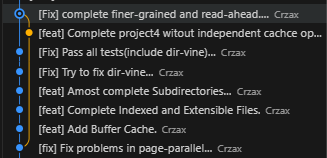
\includegraphics[width=0.5\linewidth]{figures/path.png}
    \end{figure}
    \textbf{You should think about synchronization throughout.}
\end{frame}
\begin{frame}[fragile]{a strange thing}
    To solve sector number undefined:
\begin{itemize}
    \item \begin{lstlisting}[language=C]
    bool 
    get_free_map_empty_size(void)
    {
      return bitmap_count(free_map, 0, bitmap_size(free_map), false);
    }
    \end{lstlisting}
    \item should defined in free-map.h but I define it in bitmap.h -> pass

    \item Fix warnings -> define in free-map.h
    PANIC when pintos inits.

    \item delete it -> pass 
\end{itemize}
\end{frame}
%------------------------
\begin{frame}[fragile]{Two enhancement}
\begin{itemize}
    \item \textbf{page-parallel} runs four "child-linear" processes simultaneously and waits for each to finish, checking that they return the value 0x42. It tests the system's ability to handle multiple child processes and process synchronization.

    Frame exists but supt can't be found by frame ? -> only evict frames belonging to itself.
    \item Cache lock -> each cache lock (Finer-grained lock)
\end{itemize}
\end{frame}
%----------------------
\begin{frame}{Results}
    \begin{figure}
        \centering
        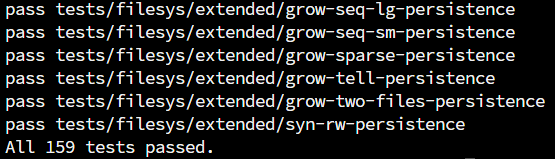
\includegraphics[width=0.8\linewidth]{figures/4.png}
        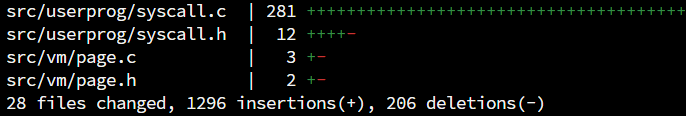
\includegraphics[width=0.8\linewidth]{figures/diff.png}
    \end{figure}
    Reference:30 files changed, 2721 insertions(+), 286 deletions(-)
\end{frame}
\begin{frame}[standout]
    Thank you!\\
  Questions?
\end{frame}

\end{document}
